\chapter{密钥生成改进方案的Niederreiter版本}
McEliece方案的提出,奠定了加解密的关键性过程。在此基础上,我们针对公钥进行了新的设计,经公钥加密的密文,在解密阶段利用私钥进行解密,上文应用的改进密钥生成方案在加解密操作是遵循McEliece方案的流程的。我们接下来将改进的密钥生成方案应用到Niederreiter方案的加解密流程,然后对其进行安全性分析和效率分析。

\section{研究动机}
从基于编码的公钥方案的研究中我们发现,大部分方案在流程上基本都是采用McEliece方案的加解密处理,但是,我们不能忽略的是McEliece方案的对偶变形,也就是Niederreiter方案。两个方案之间虽然在安全性是等价的,攻破其中一个则另一个也被认为是不安全的。但由于在公钥与私钥的存储上,两个方案并不相同,所以会有系统参数相同的情况下公钥尺寸不同的问题。公钥尺寸,一直以来是研究基于编码的加密方案的主要动机,所以如果能在安全性相同的情况下,选择公钥与私钥尺寸更小的实现方式,对方案的推行是极为有利的。

Niederreiter方案需要对明文做映射处理,也就是将明文映射成一个符合要求的差错向量,研究表明,映射算法将对整个方案的加解密速度产生不可忽略的影响,对此,我们可以引入安全哈希函数$h$,使得$h(\mathbf{e})$为随机串,如此以来,将不存在这样的缺点。关于Niederreiter方案的安全性,密码分析学者介绍了其攻击能力与方案系统参数之间的关系,为了平衡加密方案的安全性,可行性和易用性,我们有必要将改进密钥生成方案应用到Niederreiter中去。

\section{研究方向}
我们在Niederreiter方案中嵌入改进的密钥生成方案时发现,由于其私钥与McEliece方案的对偶关系,我们并不能直接应用到公钥的设计中去,但是我们修改的方向是可以确定的,就是替代原来置换矩阵的位置。

\section{方案设计}
Niederreiter方案提出以来有很多在安全性和效率性提升的变体方案,我们的改进密钥生成方案经过一些调整,是可以应用到方案中的,由此,安全性和密钥尺寸也能更好的平衡。在密钥生成流程有细节的变化,如图 \ref{fig:keygenmethodN_pdf}:

\begin{figure}[H]
	\centering
	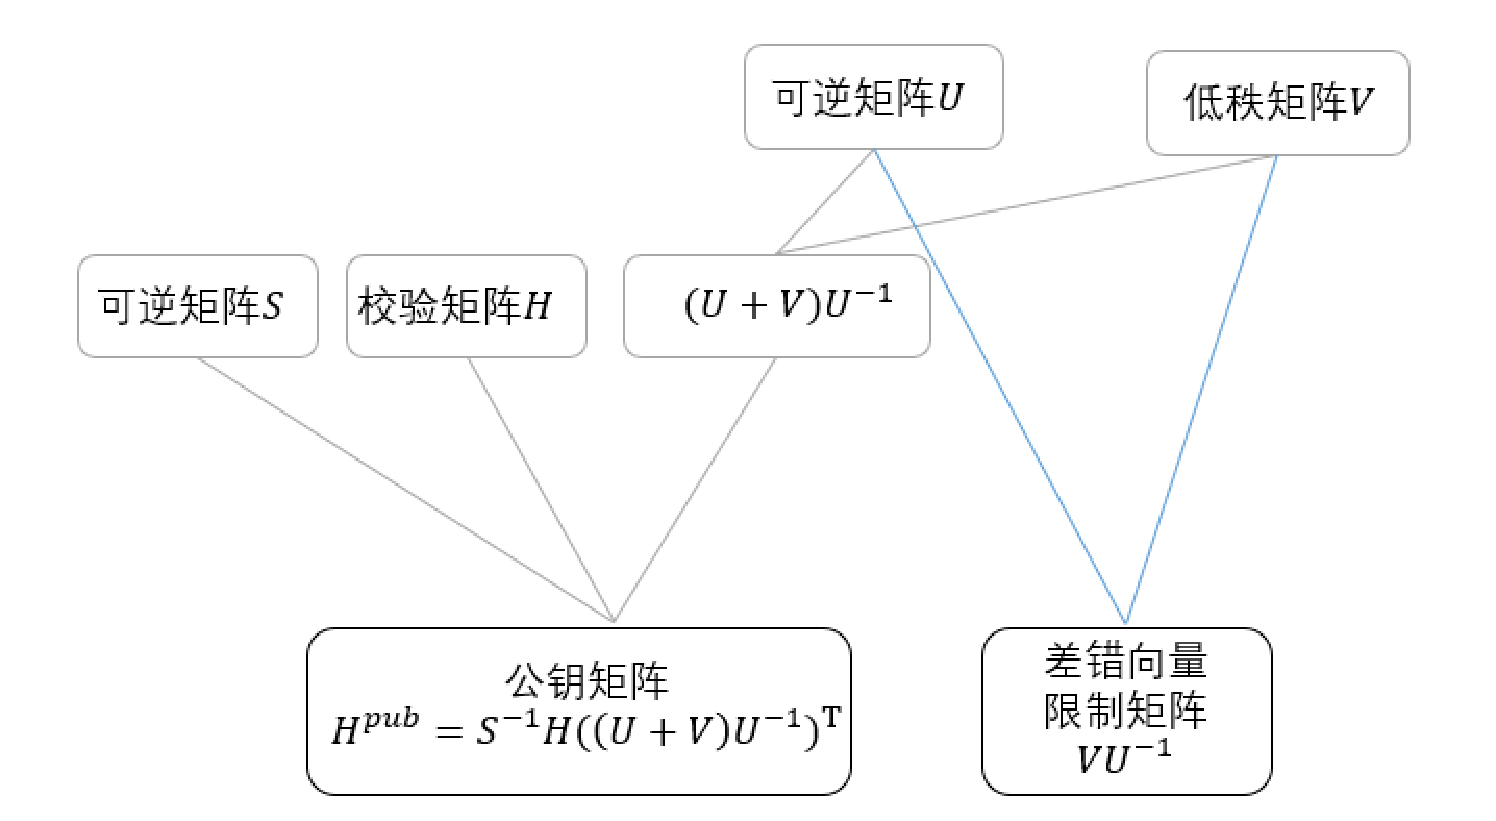
\includegraphics[width=12 cm]{fig/keygenmethodN.pdf}
	\caption{密钥生成方式} %\vspace*{-1.0cm}
	\label{fig:keygenmethodN_pdf}
\end{figure}

Niederreiter方案在混淆私钥矩阵,也就是码的校验矩阵时,同样是左乘一个可逆矩阵$S$,右乘一个置换矩阵$P$,但是接下来的问题是,公钥矩阵直接与映射成差错向量的明文做矩阵乘法,我们的改进密钥生成方案就不再适用,很明显在计算的过程中,差错向量的位数根本无法控制,后续的解密操作将一定是失败的。但是以替换置换矩阵的理论作为指导,改进密钥方案是需要做一些调整才能达到效果。具体来说,与差错向量的矩阵计算,不能扩散差错向量的位数,或者在保证一定的约束情况下,能够消除其影响。在下一节我们具体讲述改进密钥生成方案的细节设计。

\begin{breakablealgorithm}
	\small
	\renewcommand{\algorithmicrequire}{\textbf{Input:}}
	\renewcommand{\algorithmicensure}{\textbf{Output:}}
	\caption{密钥生成改进方案(Niederreiter版本)}
	\label{alg:NewKeyGenN}
	\begin{algorithmic}[1]
		\Require
		系统安全参数:$n,t \in N$,其中$t \ll n$。
		\Ensure
		公钥$(H^{pub},VU^{-1})$,私钥$(S,D_\mathcal{C},U,V)$。
		\State
		密钥生成:对于给定的参数$n$和$t$,产生下列矩阵。
		\begin{itemize}
			\item 矩阵$H$:在有限域$\mathbb{F}$上的信息位数为$k$,最小距离为$d \geq 2t + 1$的Goppa码$\mathcal{C}$的$(n - k) \times n$阶校验矩阵。
			\item 矩阵$S$:$k \times k$阶的二元随机非奇异矩阵。
			\item 矩阵$U$:$n \times n$阶的二元随机可逆矩阵。
			\item 矩阵$V$:$n \times n$阶的二元随机低秩矩阵,秩为$r$。
		\end{itemize}
		\State
		然后计算方案的公钥$H^{pub} = S^{-1}H((U + V)U^{-1})^\mathtt{T}$;接着计算另一公钥矩阵$VU^{-1}$。
		\begin{itemize}
			\item 公钥:$(G^{pub},U^{-1}V,t)$。
			\item 私钥:$(S,D_\mathcal{C},U,V)$,有效译码算法$D_\mathcal{C}$就是所用纠错码方案的陷门。
		\end{itemize}
	\end{algorithmic}
\end{breakablealgorithm}

观察公钥的设计可知,可逆矩阵$U$,与低秩矩阵$V$相加,使得满足可逆,外侧不再是右乘可逆矩阵$U$,而是右乘可逆矩阵$U^{-1}$,结果$(U + V)U^{-1}$必然也是一个可逆矩阵。于是我们就达到了以可逆矩阵替换原始Niederreiter加密方案的置换矩阵,在接下来的加解密算法中,我们

\begin{breakablealgorithm}
	\small
	\renewcommand{\algorithmicrequire}{\textbf{Input:}}
	\renewcommand{\algorithmicensure}{\textbf{Output:}}
	\caption{密钥生成改进方案加密算法(Niederreiter版本)}
	\label{alg:NeweEnN}
	\begin{algorithmic}[1]
		\Require
		公钥$(H^{pub},VU^{-1},t)$,长度为$k$的明文$\mathbf{m}$。
		\Ensure
		密文$\mathbf{c}$。
		\State
		对明文$m$,首先映射成汉明重量为$t$的差错向量$\mathbf{e} \in \mathbb{F}^n$,且满足:
		\begin{equation}
		wt(\mathbf{e})\leq t\quad \mbox{and}\quad \mathbf{e}\cdot VU^{-1} = \mathbf{0}.
		\end{equation}
		\State
		加密,产生密文:
		
		\centering $\mathbf{c} = H^{pub}\mathbf{e}^\mathtt{T}.$
	\end{algorithmic}
\end{breakablealgorithm}

类似于上一章,本次密钥生成方案需要对差错向量$\mathbf{e}$做了式 5.1的要求。式 5.1本质上与式 4.1的作用相同,要求矩阵$V$是低秩矩阵,是为了保证$VU^{-1}$的解空间足够大,使差错向量$\mathbf{e}$的有一定的随机性,避免暴力攻击。加密后的密文其实就是一个伴随式,对差错向量的约束,会使得在解码的时候,不会因为超出纠错能力而失败。

本方案的解密算法实际上类似Niederreiter方案的解密流程,具体的实现如下:

\begin{breakablealgorithm}
	\small
	\renewcommand{\algorithmicrequire}{\textbf{Input:}}
	\renewcommand{\algorithmicensure}{\textbf{Output:}}
	\caption{密钥生成改进方案解密算法(Niederreiter版本)}
	\label{alg:NewDeN}
	\begin{algorithmic}[1]
		\Require
		密文$\mathbf{c}$,私钥$(S,D_\mathcal{C},U,V)$。
		\Ensure
		明文$\mathbf{m}$。
		\State
		解密密文$\mathbf{c}$之前,首先利用私钥矩阵$S$计算:
		\begin{center}
			$S^{-1} \cdot \textbf{c} = H((U + V)U^{-1})^\mathtt{T}\mathbf{e}^\mathtt{T}.$
		\end{center}
		\State
		接着利用私钥矩阵$U$与$V$的和$(U + V)$推导上述结果:
		\begin{equation}
		\begin{aligned}
		H((U + V)U^{-1})^\mathtt{T}\mathbf{e}^\mathtt{T} &= H(\mathbf{1} +VU^{-1})^\mathtt{T}\mathbf{e}^\mathtt{T} \\
		& = H(\mathbf{e}(\mathbf{1} +VU^{-1}))^\mathtt{T} \\
		& = H(\mathbf{e} + \mathbf{e}VU^{-1})^\mathtt{T}.
		\end{aligned}
		\end{equation}
		
		\State
		观察上一步的结果,因为我们约束差错向量$\mathbf{e}$满足式 5.1,所以该结果是最多含有$t$个错误的伴随式,必然不会超过码的纠错能力,所以经过译码可以得到:
		\begin{center}
			$\mathbf{e} ^ \mathtt{T} = D_\mathcal{C}(H(\mathbf{e} + \mathbf{e}VU^{-1})^\mathtt{T}).$
		\end{center}
		
		\State
		最后,反映射可以从差错向量$\mathbf{e}$得到明文$\mathbf{m}$。		
	\end{algorithmic}
\end{breakablealgorithm}

\section{安全性分析}
对原始的Niederreiter方案的攻击,我们首先从矩阵分解攻击的角度谈起。原始Niederreiter方案中公钥共由三个矩阵部分构成,即可逆矩阵、校验矩阵、置换矩阵,如果将公钥完全分解为正确的私钥,则Niederreiter方案被完全攻破,该种暴力攻击在系统参数比较大的时候,工作因子是天文数字。更不用说,我们的改进密钥生成方案由更多的矩阵组成,且并不是向置换矩阵这样的系数矩阵,敌手采用分解的攻击方法在我们的方案中一定是无效的。除了这种攻击方式,还有以下几种常见的攻击方式。

\paragraph{信息集解码攻击}
改进的密钥生成方案在Niederreiter方案中发挥的作用,大致与McEliece方案的安全性一致。明文经过映射成的差错向量,与一个可逆矩阵的矢量计算,将很好的发挥到随机混淆作用。一些Nidderreiter方案的变体提出将公钥矩阵进行拆分,并作随机化处理,使得敌手无法获得完整的加密结果,从而不能进行有效的信息集攻击。而我们改进的密钥生成方式,也可以做拆分处理而不影响解密结果。敌手利用信息集解码攻击,总是要利用公钥加密的完整结果,进行判断进而获取密文信息,所以有必要设计可拆分的公钥,才能更好的抵御这种攻击。

\paragraph{解线性方程组攻击}
这是一种常用的攻击Niederreiter方案的方法,其思想是根据明文矢量,密文矢量及公钥矩阵的计算关系。敌手选择公钥矩阵$H^{pub}$中任意$k$个列向量,删除后只剩一个$(n - k) \times (n - k)$的公钥矩阵$(H^{pub})'$,如果$(H^{pub})'$可逆,则计算$\mathbf{c}(H^{pub})'$,否则继续选取任意$k$个列向量;然后判断$\mathbf{c}(H^{pub})'$的汉明重量,若$\mathbf{c}(H^{pub})' = t$,则破译成功,明文可以在$\mathbf{c}(H^{pub})'$对应位置补$0$即可。研究证明,其工作因子为$(n - k) ^ 3 \tbinom{n}{k} \tbinom{n - t}{n}$。针对该种攻击,我们可以利用QC-LDPC码替换Goppa码,而我们的改进密钥生成方案替换置换矩阵的部分是密集的,所以不会再导致采用稀疏矩阵容易遭受攻击的问题。

\section{效率分析}
首先从公钥尺寸方面看,公钥的构造同上一章介绍的相同,只是具体形式的不同。公钥的组成部分在求逆和矩阵计算的操作复杂度也是同上一章是一样的,这就需要我们优化系统参数,以降低公钥尺寸的影响。另外,公钥矩阵$H^{pub}$在存储的时候可以通过矩阵转换,只存取其冗余部分,这一点在McEliece方案中是做不到的。与此同时,除了我们的私钥可逆矩阵$U$,我们还有一个不可逆的私钥低秩矩阵$V$,该矩阵同样可以通过矩阵转换,只保留一个$r \times n$的矩阵进行存储,也可以进一步的缩小密钥在存储上的开销。

接下来从计算效率来看,解密操作是有序,正确且稳定的。BBCRS提出的应用Niederreiter加解密版本的方案,仍然无法避免解码失败的问题,因为两大因素,一个是矩阵$T$的平均行重或列重,会导致随机不均匀的差错向量的错误位数有可能超过码的纠错能力;而是因为公钥的混淆操作对差错向量的影响在解密阶段无法消除,只能穷举所有的结果,这种解码中重复类型的操作很容易影响密码系统的效率。幸运的是,我们都可以避免这样的问题,保持了基于编码的加密方案位运算的优势。

\section{本章小结}
本章是上一章的应用补充,从研究动机和方向做了初步的分析,得出在Niederreiter应用可以达到加解密正确性的要求。接着我们详细描述了密钥的生成算法,这里有一些细微的改动,但是基本思想是不变的。

后续在安全性和效率的分析上,我们除了与McEliece方案等价的安全性之外,说明了针对Niederreiter方案的攻击手段和提升安全性的方法。这也使得我们改进的密钥生成方案可以结合一些变体,达到安全性和效率的平衡要求。
